\section{Sparse data movement optimization}
\label{sec:approaches}
We start this section by presenting inefficiencies in current systems in the support of sparse data movement. We propose novel approaches for multipath data movement to overcome these inefficiencies.

\subsection{Inefficiency in current data movements}
For data transfers between compute nodes on the BG/Q, a message from a source to a destination traverses a single path. In the absence of congestion and network failures, default routing algorithms are used, causing the message to traverse a deterministic and single path. Figure \ref{fig:multiply}(a) depicts the single path data movement, in which one path is used other paths are idle. With dense, uniform data movement patterns where a majority of nodes and network links are involved in communications, the utilization of system resources is high. Whereas with sparse data movement patterns, only specific regions of the system are involved in communications, resulting in a low utilization of the resources.

Similarly, I/O messages such as writes as shown in Figure \ref{fig:multiply}(b) travel along a default path to default I/O nodes. When the writes  have a uniform distribution on data size and location, I/O nodes allocated for applications are used efficiently. However in sparse data movements, due to uneven distribution of data movement requests, I/O nodes and the interconnect networks suffer from an unbalanced load. The current MPI-IO implementation aggregates data to intermediate nodes, but these nodes are neither uniformly distributed nor balanced to connect to all I/O nodes. 

We next present a general approach to improve resource utilization for data movement. We then present two sub-algorithms for sparse data movements, one for among compute nodes and the other for between compute nodes and I/O nodes.

\subsection{Data movement using multiple paths}
One way to improve the utilization is to employ multiple paths. We can assign non-overlapping multiple paths for multiple messages going out from a node. Theoretically, each message would concurrently follow a non-overlapping path and the data movement therefore promises to achieve  improvement. However, at programming level, the current BG/Q system has no ability to set up paths for messages explicitly. However, we can still leverage disclosed default routing algorithms to implement concurrent data movement via multiple paths in the user-space. Thus, we can greatly simplify the deployment of our heuristics.

\begin{figure}[!htb]
\vspace{-0.1in}
\centering
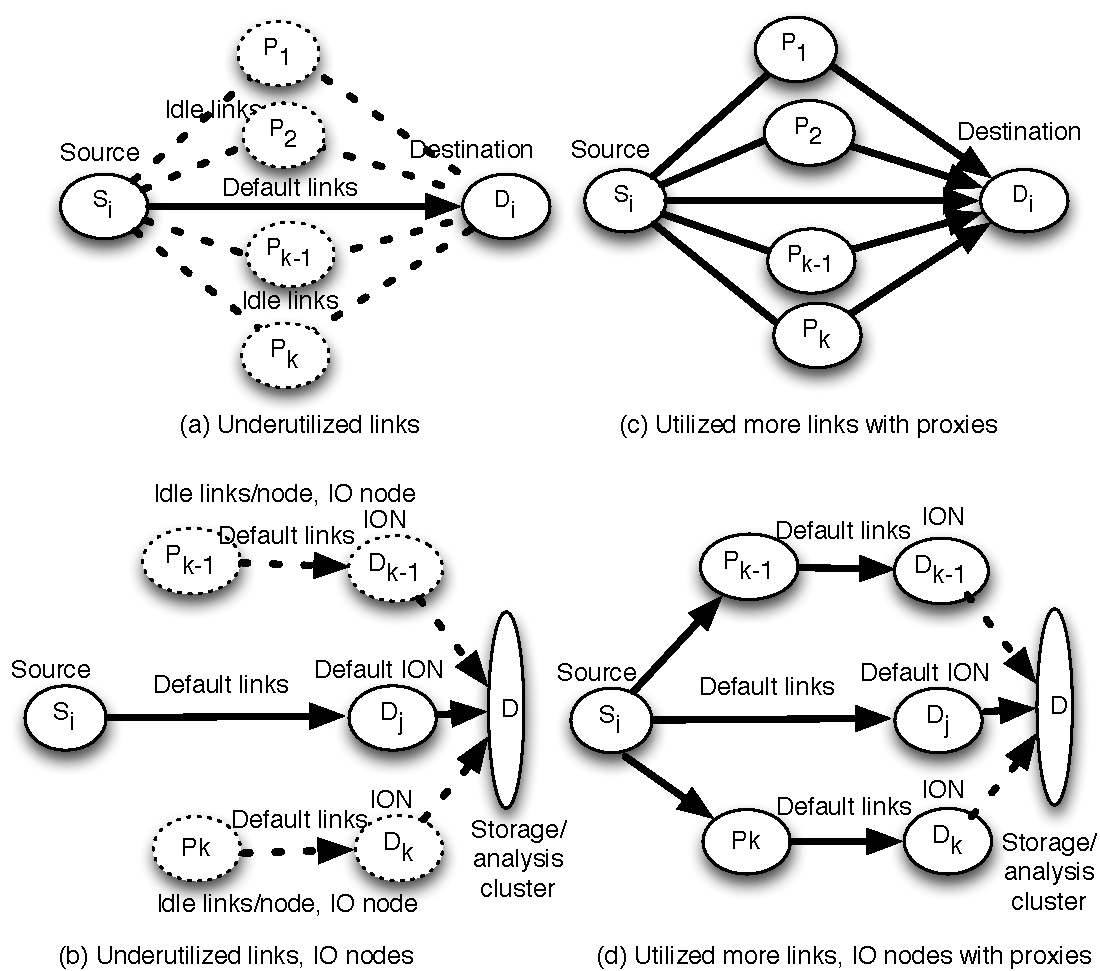
\includegraphics[scale=0.5]{figures/multiply}
\vspace{-0.2in}
\caption{Data transfer with and without proxies}
\vspace{-0.1in}
\label{fig:multiply}
\end{figure}

In order to route data along multiple paths on a single-path-allowed system, we introduce intermediate nodes which are compute nodes where the application runs to serve an additional purpose of routing data. Leveraging the default routing, we first route data from sources to the intermediate nodes and then from intermediate nodes to destinations. As shown in Figure \ref{fig:multiply}(c), by adding intermediate nodes we increase the number of paths to move data between nodes, overcoming the system limitation of a deterministic single path for data movement. The  routing function on the intermediate nodes does introduce little additional overheads, and we assume that future systems might provide such functionality at the node level for a multipath routing.  Knowing the routing policy a priori, we choose the locations of intermediate nodes to minimize the shared links and therefore maximize the data movement throughput. In Figure \ref{fig:multiply}(d), by adding the intermediate nodes we increase the number of I/O nodes and accordingly balance I/O workload. 
We also propose a mechanism that leverages interconnect topology and distributes intermediate nodes dynamically among all I/O nodes to achieve significant improvement in I/O. 

Implementing multipath data movement using intermediate nodes requires several steps.
\begin{itemize}
\item Calculate the message sizes to see if using intermediate nodes benefits performance and how to use them.
\item Determine the number and location of intermediate nodes.
\item Transfer data using multipaths from sources to destinations via intermediate nodes.
\end{itemize}

In the next sections, we realize the above steps for sparse data movement among compute nodes and sparse data movement to I/O.

\subsection{Sparse data movement between groups of compute nodes}
In this subsection, we present an algorithm to select the number and the locations of intermediate nodes together with multipath data movement between two groups of compute nodes. This is critical for data coupling in multiphysics codes. Intermediate nodes will be referred to as proxies for the rest of the paper. 

We start with selecting number of proxies. Each proxy adds an additional non-overlapping data movement path,. Adding more paths reduces congestion and improves the transfer time. However, as we introduce proxies, additional overhead, and hence time, is also introduced due to the additional processing and buffering at the proxy. Therefore performance gained by introducing proxies needs to be at least enough to compensate the extra time caused by introducing them. We model the time for data movement from one node's memory to another node's memory using remote direct memory access (RDMA) as follows.

\begin{figure}[!htb]
\vspace{-0.1in}
\centering
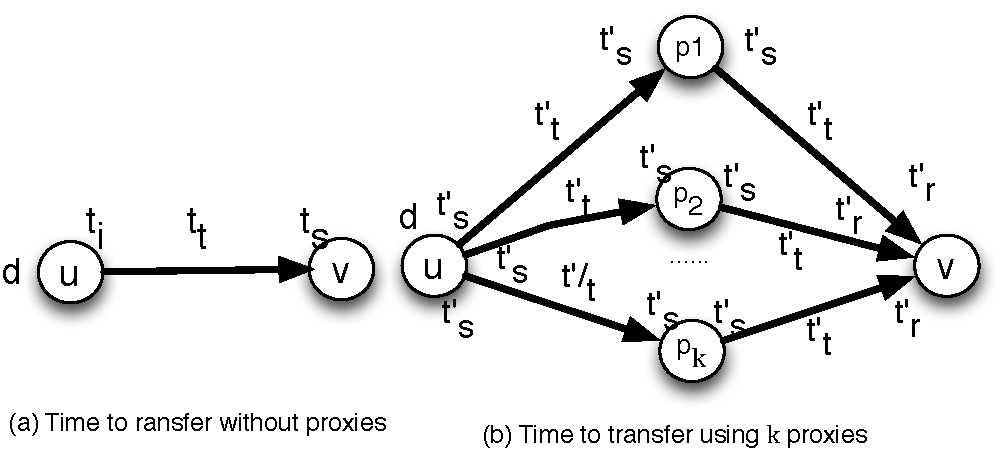
\includegraphics[scale=0.5]{figures/transfer_time.pdf}
\vspace{-0.2in}
\caption{Time to transfer in case of with and w/o proxies}
\vspace{-0.1in}
\label{fig:proxies}
\end{figure}
For data transfer, communication delay is composed of processing delay, transmission delay, queueing delay and propagation delay. To make it simple, we model the delays into 3 variables: time for processing, queueing and injecting at sender node t$_s$, time to transfer data t$_t$ and time for processing, queueing and storing at receiver node t$_r$. The time is depicted in Figure \ref{fig:proxies}. The total time to transfer a message of size d from sender u to receiver v therefore is:

\begin{equation}
t = t_s + t_t + t_r
\end{equation}

In which:
\begin{itemize}
\item $t$: Total time to transfer.
\item $t_s$: Time to process, queue and inject a message of size d into the network at sender
\item $t_t$: Time to actually transfer a message of size d from sender' network interface to receiver's network interface.
\item $t_r$: Time to process, queue and store a message of size $d$ from network to memory at receiver.
\end{itemize}

In the case of using k paths with k proxies, the data size each path carries would be $\frac{d}{k}$, assuming equal split. Data is transferred in two steps from the sender to proxies, completely stored at the proxies, and then moved from the proxies to the receiver. Each proxy becomes an extra sender and receiver. Thus, we need to account for this additional processing and buffering at proxy endpoints. The time for transfer in each hop can be considered approximately the same. Hence, total time to transfer data is:
\begin{equation}
t' = 2(t'_s + t'_t + t'_r) %2(\frac{t'_i}{k} + \frac{t'_t}{k} + \frac{t'_s}{k}) = 2\frac{t'_i + t'_t + t'_s}{k}
\end{equation}

In which:
\begin{itemize}
\item $t'$: Total time to transfer.
\item $t'_s$: Time to process, queue and inject a message of size d/k into the network at sender
\item $t'_t$: Time to actually transfer a message of size d/k from sender's network interface to receiver's network interface.
\item $t'_r$: Time to process, queue and store a message of size d/k from network to memory at receiver.
\end{itemize}

The ratio of total time for two data transfer methods is:
\begin{equation}
\frac{t'}{t} = \frac{2(t'_s + t'_t + t'_r)}{t_s + t_t + t_r} 
\end{equation}

As we split a message into k messages, time to transfer data is reduced linearly. However, the time to inject and  to store do not. Actually the total time to inject or store $k$ messages of size d/k each is at least the time for one single message size $d$. This is due to overheads to process and buffer the data. Therefore:

\begin{equation}
t'_s \ge \frac{t_s}{k}; \; 
t'_t = \frac{t_t}{k}; \; 
t'_r \ge \frac{t_r}{k}\; 
\end{equation}

The equalities happen only when message size is greater than a threshold. For the message size greater than  the threshold, we have:
\begin{equation}
\frac{t'}{t} = \frac{2(t'_s + t'_t + t'_r)}{t_s + t_t + t_r} = \frac{2(\frac{t_s}{k} + \frac{t_t}{k} + \frac{t_r}{k})}{t_s + t_t + t_r} = \frac{2}{k}
\end{equation}

Thus, to get benefit from setting up proxies, we need to have at least 3 proxies per data transfer, and we can improve $k/2$ times throughput.

For small messages, as $t'_s \gg t_s/k$ and $t'_r t_r/k$, we need a much greater value of k to get benefit from setting up proxies, which is usually not feasible. In Section \ref{sec:microbenchmarks}, we show threshold values computed based on experiments at which for smaller messages, direct transfer is better than proxy-based transfer, and for bigger messages, proxy-based transfer is better. Therefore, proxy-based techniques should be used for intensive sparse data movements when the size of message is greater than a threshold.

With respect to the placement of the proxies, we need to choose positions of the proxies to minimize link sharing since we know routing paths in advance. It is difficult and sometimes impossible to choose proxies as the number of nodes involved in data movement increases. We develop an heuristic algorithm to check if it is feasible to implement proxies and to find the number and position of these proxies. The BG/Q is connected via 5D torus, however to simplify the algorithm illustration and description, we depict the data movement of the algorithm for 2D mesh as in Figure \ref{fig:groxies}. The 5D torus or any k-D torus would work in the same way. In our work, we assume that regions of a cluster that need to communicate data are contiguous. This assumption is valid under many multi-physics applications such as Community Earth System Model \cite{CESM:Collins} as processes of an application are usually mapped contiguously to improve intra-group communication. We also assume that the network is dedicated with no background communication from other applications.

\begin{figure}[!htb]
\vspace{-0.1in}
\centering
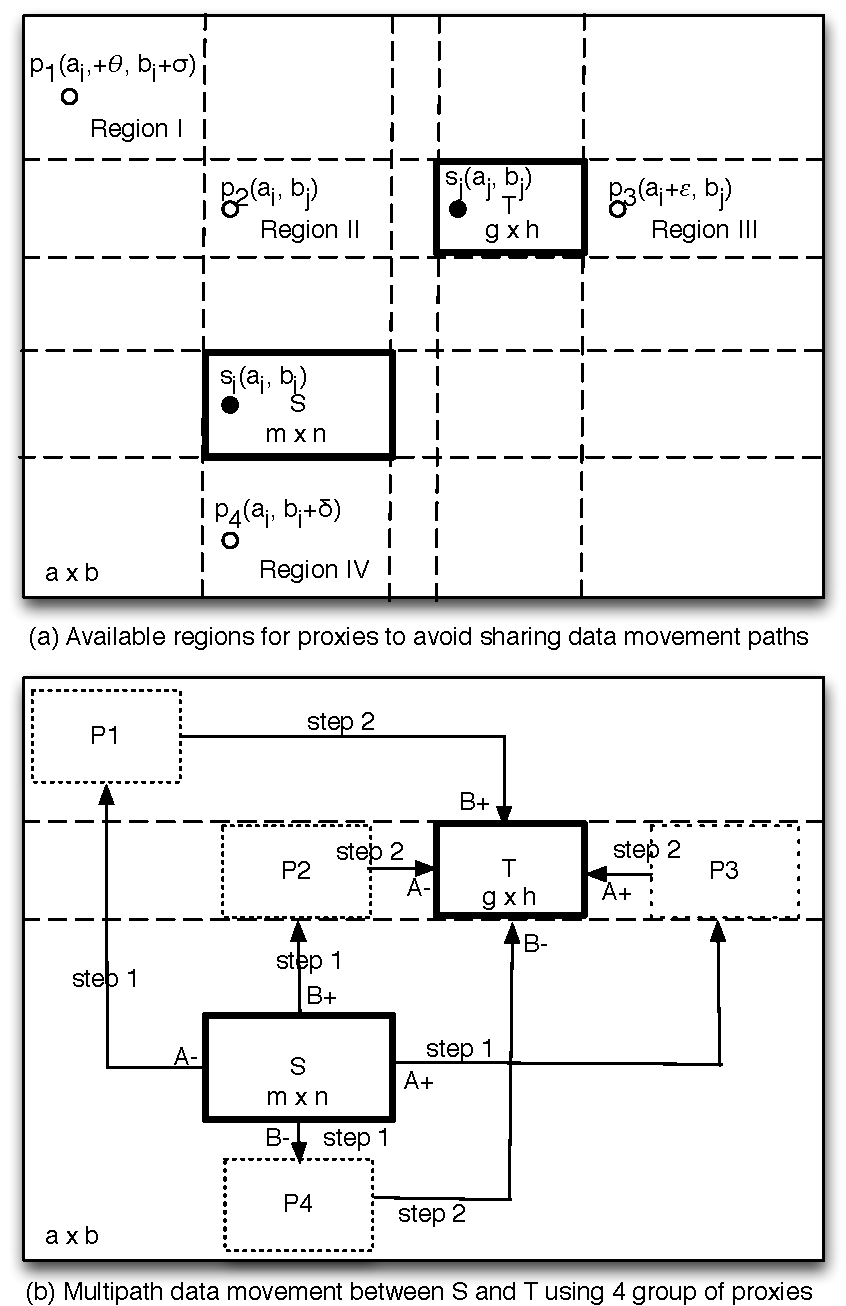
\includegraphics[scale=0.5]{figures/groxies.pdf}
\vspace{-0.1in}
\caption{Using 4 groups of proxies at 4 directions to transfer data between 2 groups in 2 steps}
\vspace{-0.2in}
\label{fig:groxies}
\end{figure}

The Figure \ref{fig:groxies} depicts a 2D allocation of \textit{a} x \textit{b} mesh topology for multi-physics application. In the 2D mesh, data is routed horizontally (A direction) first and then vertically (B direction). Two physics codes S and T running at 2 regions of the cluster are data coupled (i.e., T needs data from S to complete a computation.) Region S has the size \textit{m} x \textit{n}, while T has the size \textit{g} x \textit{h}. We assume that each node has approximately the same amount of data and each destination receives approximately the same amount of data.

\begin{itemize}
\item S: Set of source nodes, size $|S|$ = m*n = M
\item T: Set of destination nodes, size $|T|$ = g*h = N
\item P$_i$: Proxies nodes of source node s$_i$.
\item L: Number of dimensions of the network.
\item $coord_{il}$: Coordinate of a node i, dimension l
\item Each s$_i$ $\in$ S:
\begin{itemize}
\item Has targets T$_i$ and proxies P$_i$.
\item Data size d$_i$ at s$_i$ is sent to set of t$_i$ in T$_i$. s$_i$ sends d$_{i}$ to t$_i$ through p$_i$

\end{itemize}
\end{itemize}

Here we develop a heuristic algorithm for data movement between multiple sources and multiple destinations using multiple paths leveraging known  data routing algorithms. Note that the default routing algorithms here is order-based and given the torus size of the allocation, message size and coordinates of source and destination are known a priori. The algorithm is described in Algorithm \ref{Alg:groxies}.

\begin{algorithm}
\caption{Algorithm for data movement between 2 groups of nodes}
\begin{algorithmic}

\STATE \textbf{I. Init}
\STATE Exchange coordinations of the sources and destinations.
\FOR {each node s$_i$ in S with i = 1..M}
\STATE P$_i$ = $\varnothing$, T$_i$ = $\varnothing$.
\STATE Adding its destination nodes t$_j$ into T$_i$.
\ENDFOR

\STATE \textbf{II. Find Proxies}
\FOR {each source node s$_i(\{coord_{il}\})$ in S}
\FOR {each its destination node $t_j({coord_{jl}})$ in T$_i$}
\STATE Sort the dimensions by routing order.
\FOR{each dimension l with l = 1..L in the sorted order}
\STATE Check 2 candidates: c$_p$ and c$_n$ on the + and - on the l direction of the s$_i$. %$(a_i, b_j), (a_i+\epsilon, b_j), (a_i, b_i+\delta), (a_i+\theta, b_i+\sigma$) w.r.t $(a_j-a_i)*(a_j-(a_i+\epsilon)) < 0, (b_i-b_j)*(b_i-(b_i+\delta)) < 0, (b_j-b_i)*(b_j-(b_i+\sigma)) < 0, (a_i-a_j)*(a_i-(a_i+\theta)) < 0$.
\STATE If a candidate is available, add it into P$_i$.
\ENDFOR
\ENDFOR
\IF {$|Pi| < 3$} \STATE Exit. \ENDIF
\ENDFOR

\STATE \textbf{III. Multipath Data Movement}
\STATE Phase 1: At each node s$_i$ in S:
\FOR{\textbf{each} p$_{ij}$ in P$_i$}
\STATE Send data to p$_{ij}$ with size d$_{ij}$.
\ENDFOR
\STATE Phase 2: At each proxy p$_{ij}$:
\STATE Send data to the destination.
\end{algorithmic}
\label{Alg:groxies}
\end{algorithm}

Our algorithm includes 3 parts: In the \textbf{Init} part, we exchange the coordinates of all sources and destinations. After that, each node s$_i$ initializes its empty sets of proxies P$_i$ and destinations T$_i$. The destinations of s$_i$ are then added to the T$_i$. If the set of sources and destinations are known a priori, an application only needs to run \textbf{Init} once. In the \textbf{Find Proxies} part, each source node checks 2*L possible candidates along L destinations. In the 2-dimension mesh, each node has 4 directions of +A, -A, +B and -B to send/receive data. There are 4 regions marked from I to IV in Figure \ref{fig:groxies}(a) to search for possible proxies that guarantee non-overlapping concurrent data movements. We can search for 4 proxies in the 4 regions with offsets from the source and the destination represented by values of $\epsilon, \delta, \theta, \sigma$. This is to make sure that 4 proxies are in the 4 distinct directions for both outgoing and incoming transfers.  Due to small torus size, searching for these values are not time consuming. If those values exist, we then add the proxies into the list P$_i$. If each source node can have at least 3 proxies then we continue the next part. Otherwise, we discard since there is no benefit to setup proxies. In the last part, \textbf{Multipath Data Movement}, we first move data from source nodes to proxies and then from proxies to destination nodes. To extend for L dimensions, we need to search for 2L directions (both negative and positive directions per each dimension) to find at most 2L proxies.

The algorithm is distributed and runs at every node. Except for gathering all coordinates at the beginning, the remainder of the algorithm executes without waiting (synchronizing) for all other nodes. The running time of the algorithm is O(M*N*L). However, due to small sizes of most networks, the actual time to compute the routes is small. Overall, the overhead for searching for proxies is negligible.

\subsection{Sparse data movement between compute nodes and I/O nodes}
\label{sec:stagingandio}
Each compute node is associated with a default I/O node. Therefore, we need to have at least one intermediate node for each I/O node available in the allocated partition to use the I/O node.
Depending on the data size, we may need more than one intermediate node per I/O node. Also, these intermediate nodes need to be uniformly distributed to avoid data congestion when sending data from compute nodes to intermediate nodes. Thus, to calculate the number of intermediate nodes needed, we need to know total size of data, available I/O nodes, location of compute nodes and their default I/O node. We uniformly distribute these intermediate nodes to the I/O nodes. Data is then aggregated from compute nodes to these intermediate nodes. In this way, an I/O node for which all of its compute nodes do not have data or have small size of data still receives I/O requests with approximately equal amount of data as intermediate nodes are chosen among its compute nodes. As these intermediate nodes aggregate data from a large number of nodes, we call them aggregators. The approach is presented in Algorithm \ref{Alg:aggregation}.

\begin{algorithm}
\caption{Algorithm for I/O data movement}
\begin{algorithmic}
\STATE \textbf{I. Init}
\STATE Define the smallest size of data aggregated at each aggregator S.
\STATE Each node queries its coordinates and its default I/O node.
\STATE Calculate total number of IO nodes for the partition: n$_{io}$.
\STATE List number of aggregators may be needed per I/O nodes: P = \{1,2,4..., 128\}.
\FOR {each value num\_agg in the list P}
\STATE Calculate the positions of aggregators based on the number of aggregators (num\_agg):
\STATE Divide the pset along 5 dimensions by factors nA, nB, nC, nD, nE such as nA*nB*nC*nD*nE = num\_agg to create blocks.
\STATE For each block, choose the first one as the aggregator.
\STATE Save the aggregators for later use.
\ENDFOR

\STATE \textbf{II. Redistribute data}
\STATE Reduce and broadcast the total size of data need to be written: T = $\sum_{i=1}^{n}d_i$.
\STATE Calculate the number of aggregators needed per pset: num\_agg = T/S/n$_{io}$.
\STATE Based on num\_agg select the list of the aggregators from pre-created list and broadcast it to nodes having data.
\STATE Each nodes having data sends its data to its chosen aggregator(s).
\STATE Selected aggregators send data out through I/O nodes.
\end{algorithmic}
\label{Alg:aggregation}
\end{algorithm}

In the first part of the algorithm, \textbf{Init}, the algorithm queries all the information of I/O nodes, coordinates of compute nodes and its default I/O node. It then precomputes all possible aggregators and their location at all processes. The data is stored in list P, used later for redistributing data. To compute P, it divides the partition into equal blocks. It can create a subcomm using MPI\_Comm\_create for each sub-network and select the MPI rank 0 of the subcomm as the aggregator of the subnetwork. In the second part, \textbf{Redistribute data}, depending on total size of data for each I/O request, it selects appropriate aggregators and then carries multipath data movement.

Since all the necessary information is queried and computed once at the beginning, we save time at each I/O request. At each I/O request, the only information needed to gather is total size of data. The aggregators are chosen dynamically and distributed uniformly to balance the load among I/O nodes.

\subsection{Pipeline technique for data movement}
In the graph model, data is transferred from a source to destination through proxies without extra delay. As we have to transfer data from the source node to proxies first, then from the proxies to the destination, we need to store data at a proxy. If we store entire message at the proxy, it takes time to wait until the entire message arrives and  then start injecting the message into network to the next proxy. To reduce the time to wait, we cut the message into smaller messages and transfer messages using pipeline such that storing messages and sending messages at a proxy can run concurrently. %Figure \ref{} depicts the process.

%\begin{figure}[!htb]
%\centering
%\includegraphics[scale=0.5]{figures/pipeline.pdf}
%\caption{Using pipelining technique to eliminate the waiting time at proxy}
%\label{fig:pipeline}
%\end{figure}

For each proxy, requests to wait for data is posted at the beginning. After that, the proxy needs to iterate through the list of requests while checking if data is ready to forward. To implement the pipeline, we create two threads at each proxy: one thread for receiving data and the other for forwarding data. A message is cut into smaller message with certain size called window size. The size of window depends on message size and is determined based on experiments. Within each message we embed the information of how data would be process at the next node such as destination, address of the message in the destination's buffer, the path Id that next node should use to forward the message. The pipeline technique can be used in any system and yields significant improvement as we show in section \ref{sec:microbenchmark}. However, with small messages, we still suffer performance degradation. This is because the control overhead in small message is significantly large compared to the message size itself.

In the following sections, we present our study on Mira Blue Gene/Q to show the efficacy of our solutions.